\section{Versuchsaufbau und Durchf"uhrung} % (fold)
\label{sec:durchfuehrung}

\subsection{Direkte Messung der Leerlaufspannung} % (fold)
\label{sub:direkte_messung_der_leerlaufspannung}

\begin{figure}[!h]
	\centering
	\includegraphics[width = [10cm]]{img/Monozelle.PNG}
	\caption{Schaltbild zur direkten Messung der Leerlaufspannung. \cite{anleitung}}
	\label{aufgabea}
\end{figure}

Die Schaltung wird nach Abb.\ref{aufgabea} aufgebaut. Der Widerstand $R_\mathrm{a}$ entspricht hierbei dem Eingangswiderstand $R_\mathrm{v}$ des hochohmigen Spannungsmessger"ates.
Es werden $U_\mathrm{k}$ und $R_\mathrm{v}$ notiert.

\subsection{Messung der Leerlaufspannung und des Innenwiderstandes mittels eines variablen Widerstandes} % (fold)
\label{sub:messung_der_leerlaufspannung_mittels_eines_variablen_widerstandes_}

\begin{figure}[!h]
	\centering
	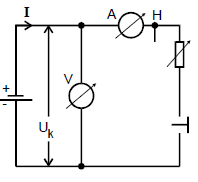
\includegraphics[width = 10cm]{img/b.PNG}
	\caption{Messchaltung zur Bestimmung von $U_\mathrm{0}$ und $R_\mathrm{i}$ \cite{anleitung}.}
	\label{aufgabeb}
\end{figure}

Die Schaltung wir nach Abb. \ref{aufgabeb} aufgebaut.
Der variable Belastungswiderstand liegt dabei in einem Bereich von $\SI{0}{\ohm}$ bis $\SI{50}{\ohm}$. Es werden die Klemmenspanung $U_\mathrm{k}$ in abh"angigkeit von dem Belastungsstrom $I$ und 10 verschiendenen Belastungswiderst"anden $R_\mathrm{a}$ aufgenommen.

\subsection{Messung der Leerlaufspannung und des Innenwiderstandes mittels eines variablen Widerstandes und einer Gegenspannung} % (fold)
\label{sub:messung_der_leerlaufspannung_mittels_eines_variablen_widerstandes_}

\begin{figure}[!h]
	\centering
	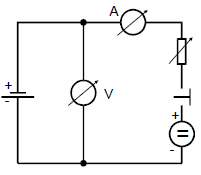
\includegraphics[width = 10cm]{img/c.PNG}
	\caption{Messchaltung zur Bestimmung von $U_\mathrm{0}$ und $R_\mathrm{i}$ mittels einer Gegenspannung\cite{anleitung}.}
	\label{aufgabec}
\end{figure}

